% Adaptado de Semana 07 Clase 01 (2025-A), con motivación geométrica.
\documentclass[compacto,10pt]{pubciencias-notas}
\usepackage{comandosEPN}
\usepackage{tikz}
\usetikzlibrary{babel}
\autor{Departamento de Formación Básica}
\materia{Álgebra Lineal}
\nota{Semana 05 Clase 02}
\fecha{Semestre 2026-B}
\logouno[1.1cm]{Logo_EPN.eps}
\logodos[1.7cm]{Logo_DFB.eps}
\definecolor{colordef}{cmyk}{0.81,0.62,0.00,0.22}

\begin{document}
\encabezado
\vspace*{-8mm}
\setcounter{section}{3}
\section{Espacios vectoriales}
\subsection{Motivación: operar con desplazamientos}

Un desplazamiento en el plano se representa mediante un vector
$u=(u_1,u_2)$. Podemos dibujarlo como una flecha desde el origen hasta el punto
$(u_1,u_2)$; trasladar la flecha sin cambiar su dirección, sentido ni longitud
representa el mismo desplazamiento. En esta clase escribiremos los vectores
como tuplas; en un producto matricial los interpretaremos como columnas.

\begin{ejem}[Componer, escalar e invertir un movimiento]
    Sean $u=(2,1)$ y $v=(1,3)$. La suma compone los desplazamientos:
    \[
        u+v=(3,4).
    \]
    El producto por un número real cambia la escala del movimiento:
    \[
        2u=(4,2),\qquad -u=(-2,-1),\qquad 0u=(0,0).
    \]
    El vector $-u$ permite regresar después de ejecutar $u$;
    el vector cero representa no desplazarse.
\end{ejem}

\begin{center}
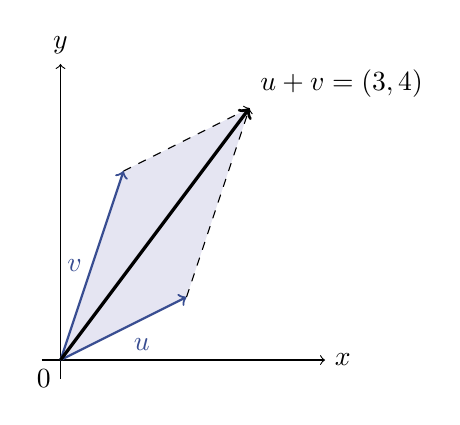
\begin{tikzpicture}[scale=0.8]
    \draw[->] (-0.3,0)--(4.2,0) node[right] {$x$};
    \draw[->] (0,-0.3)--(0,4.7) node[above] {$y$};
    \fill[colordef!10] (0,0)--(2,1)--(3,4)--(1,3)--cycle;
    \draw[->,thick,colordef] (0,0)--(2,1) node[midway,below right] {$u$};
    \draw[->,thick,colordef] (0,0)--(1,3) node[midway,left] {$v$};
    \draw[->,dashed] (2,1)--(3,4);
    \draw[->,dashed] (1,3)--(3,4);
    \draw[->,very thick] (0,0)--(3,4) node[above right] {$u+v=(3,4)$};
    \node[below left] at (0,0) {$0$};
\end{tikzpicture}
\end{center}

\noindent\textbf{Para discutir.} Si primero ejecutamos $v$ y después $u$,
¿cambia el desplazamiento final? ¿Qué representan $\frac12u$ y $-2u$?

Hasta ahora podemos movernos por todo el plano. Nos preguntamos:
\textbf{¿qué conjuntos de movimientos permiten sumar y cambiar la escala
sin salir de ellos?}

\subsection{Rectas y planos que contienen al origen}

\begin{ejem}[Moverse por una recta]\label{sem05cl02:recta}
    Supongamos que los movimientos deben seguir la dirección $u=(2,1)$.
    El conjunto de desplazamientos permitidos es
    \[
        L=\{t(2,1):t\in\R\}=\{(x,y)\in\R^2:x-2y=0\}.
    \]
    Contiene $u$, $2u$, $-u$ y el vector cero. Para comprobar que dos
    movimientos cualesquiera de $L$ pueden componerse sin salir de la recta,
    escribimos $p=su$ y $q=tu$, con $s,t\in\R$. Entonces
    \[
        p+q=(s+t)u\in L,\qquad
        \lambda p=(\lambda s)u\in L\quad\text{para todo }\lambda\in\R.
    \]
    Estas igualdades justifican la estabilidad para todos los movimientos
    y todas las escalas, no solo para los vectores que dibujamos.
\end{ejem}

\begin{center}
\begin{minipage}[t]{0.47\textwidth}
\centering
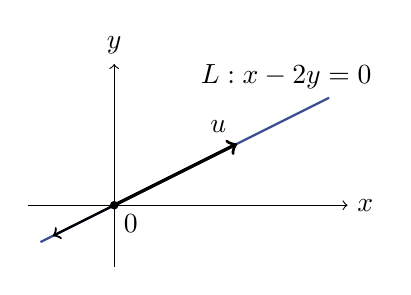
\begin{tikzpicture}[scale=0.78]
    \draw[->] (-1.4,0)--(3.8,0) node[right] {$x$};
    \draw[->] (0,-1)--(0,2.3) node[above] {$y$};
    \draw[colordef,thick] (-1.2,-0.6)--(3.5,1.75);
    \draw[->,very thick] (0,0)--(2,1) node[above left] {$u$};
    \draw[->,thick] (0,0)--(-1,-0.5);
    \fill (0,0) circle (2pt) node[below right] {$0$};
    \node at (2.8,2.1) {$L:x-2y=0$};
\end{tikzpicture}

La recta contiene al vector cero.
\end{minipage}
\hfill
\begin{minipage}[t]{0.47\textwidth}
\centering
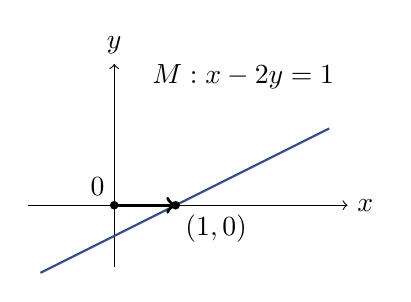
\begin{tikzpicture}[scale=0.78]
    \draw[->] (-1.4,0)--(3.8,0) node[right] {$x$};
    \draw[->] (0,-1)--(0,2.3) node[above] {$y$};
    \draw[colordef,thick] (-1.2,-1.1)--(3.5,1.25);
    \draw[->,very thick] (0,0)--(1,0);
    \fill (1,0) circle (2pt) node[below right] {$(1,0)$};
    \fill (0,0) circle (2pt) node[above left] {$0$};
    \node at (2.1,2.1) {$M:x-2y=1$};
\end{tikzpicture}

La recta trasladada no contiene al cero.
\end{minipage}
\end{center}

En cambio, $M=\{(x,y):x-2y=1\}$ contiene $(1,0)$, pero no contiene su
múltiplo $0(1,0)=(0,0)$. Por tanto, al permitir todas las escalas,
podemos salir de $M$.

\begin{ejem}[Moverse por un plano del espacio]\label{sem05cl02:plano}
    Consideremos los desplazamientos que satisfacen
    \[
        P=\{(x,y,z)\in\R^3:x+y-z=0\}.
    \]
    Los vectores $a=(1,0,1)$ y $b=(0,1,1)$ pertenecen a $P$;
    también $a+b=(1,1,2)$, $-a$ y el vector cero.
    Al despejar $z=x+y$, obtenemos
    \[
        P=\{(s,t,s+t):s,t\in\R\}
         =\{s(1,0,1)+t(0,1,1):s,t\in\R\}.
    \]
    Esta descripción utiliza dos variables libres, como en los sistemas
    homogéneos de la semana 03.
\end{ejem}

\begin{center}
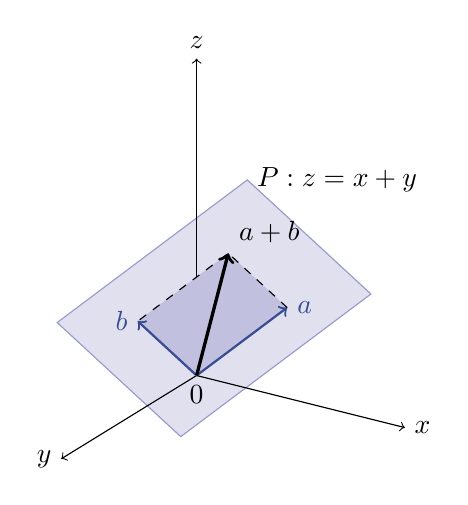
\begin{tikzpicture}[x={(1cm,-0.25cm)},y={(-0.65cm,-0.4cm)},z={(0cm,1cm)},scale=1.15]
    \filldraw[fill=colordef!12,draw=colordef!45]
        (-0.5,-0.5,-1)--(1.6,-0.5,1.1)--(1.6,1.6,3.2)--(-0.5,1.6,1.1)--cycle;
    \draw[->] (0,0,0)--(2.3,0,0) node[right] {$x$};
    \draw[->] (0,0,0)--(0,2.3,0) node[left] {$y$};
    \draw[->] (0,0,0)--(0,0,3.5) node[above] {$z$};
    \fill[colordef!25] (0,0,0)--(1,0,1)--(1,1,2)--(0,1,1)--cycle;
    \draw[->,thick,colordef] (0,0,0)--(1,0,1) node[right] {$a$};
    \draw[->,thick,colordef] (0,0,0)--(0,1,1) node[left] {$b$};
    \draw[dashed] (1,0,1)--(1,1,2)--(0,1,1);
    \draw[->,very thick] (0,0,0)--(1,1,2) node[above right] {$a+b$};
    \node[below] at (0,0,0) {$0$};
    \node[right] at (1.6,1.6,3.2) {$P:z=x+y$};
\end{tikzpicture}

\small Se muestra una porción del plano; este se prolonga indefinidamente.
\end{center}

Para comprobar la estabilidad en general, sean $p,q\in P$ y $\lambda\in\R$.
Como $p_1+p_2-p_3=0$ y $q_1+q_2-q_3=0$, se cumple
\[
    (p_1+q_1)+(p_2+q_2)-(p_3+q_3)=0,
    \qquad \lambda p_1+\lambda p_2-\lambda p_3=0.
\]
Por tanto, $p+q$ y $\lambda p$ también pertenecen a $P$.

\noindent\textbf{Complete y contraste.} El plano $Q=\{(x,y,z):x+y-z=1\}$
no contiene al vector cero. Si $p,q\in Q$, ¿cuánto vale
$(p_1+q_1)+(p_2+q_2)-(p_3+q_3)$? ¿Pertenece $p+q$ a $Q$?

\subsection{Definición de espacio vectorial real}

Los ejemplos anteriores comparten una estructura: sus elementos pueden
sumarse y multiplicarse por escalares, respetando ciertas reglas.

\begin{defi}[Espacio vectorial real]\label{sem05cl02:espacio}
    Un conjunto no vacío $V$, con operaciones de suma
    $V\times V\to V$ y producto escalar $\R\times V\to V$, es un
    \textbf{espacio vectorial real} si, para todo $u,v,w\in V$ y
    $\alpha,\beta\in\R$, se cumplen:
    \begin{enumerate}
        \item \textbf{Asociatividad de la suma:} $(u+v)+w=u+(v+w)$.
        \item \textbf{Conmutatividad de la suma:} $u+v=v+u$.
        \item \textbf{Neutro aditivo:} existe $0_V\in V$ tal que $u+0_V=u$.
        \item \textbf{Inverso aditivo:} para cada $u$ existe $-u\in V$
              tal que $u+(-u)=0_V$.
        \item \textbf{Distributividad sobre vectores:}
              $\alpha(u+v)=\alpha u+\alpha v$.
        \item \textbf{Distributividad sobre escalares:}
              $(\alpha+\beta)u=\alpha u+\beta u$.
        \item \textbf{Compatibilidad del producto escalar:}
              $\alpha(\beta u)=(\alpha\beta)u$.
        \item \textbf{Identidad del producto escalar:} $1u=u$.
    \end{enumerate}
    Los elementos de $V$ se llaman \textbf{vectores}; los números reales
    que los multiplican se llaman \textbf{escalares}.
\end{defi}

\begin{advertencia}
    Las operaciones deben ser \textbf{cerradas}: si $u,v\in V$ y
    $\lambda\in\R$, entonces $u+v\in V$ y $\lambda u\in V$.
    No basta con que las operaciones puedan calcularse en un conjunto mayor.
\end{advertencia}

Geométricamente, el neutro representa no moverse, el inverso permite regresar
y la distributividad expresa que escalar un recorrido compuesto equivale
a escalar cada desplazamiento y después sumarlos.

\begin{ejem}[El espacio $\R^n$ con sus operaciones usuales]
    Para $u=(u_1,\ldots,u_n)$ y $v=(v_1,\ldots,v_n)$, se define
    \[
        u+v=(u_1+v_1,\ldots,u_n+v_n),\qquad
        \alpha u=(\alpha u_1,\ldots,\alpha u_n).
    \]
    Estas operaciones son cerradas. El neutro es $(0,\ldots,0)$ y el inverso
    de $u$ es $(-u_1,\ldots,-u_n)$. Las otras identidades se verifican por
    componentes mediante las propiedades de los números reales.
    Por ejemplo, en $\R^2$,
    \begin{align*}
        \alpha(u+v)
        &=\bigl(\alpha(u_1+v_1),\alpha(u_2+v_2)\bigr)\\
        &=\bigl(\alpha u_1+\alpha v_1,\alpha u_2+\alpha v_2\bigr)
         =\alpha u+\alpha v.
    \end{align*}
    \textbf{A su turno:} justifique $1u=u$ y
    $(\alpha+\beta)u=\alpha u+\beta u$ con vectores generales de $\R^2$.
\end{ejem}

\subsection{Cómo verificar nuestros ejemplos geométricos}

\begin{prop}[Criterio para subconjuntos de $\R^n$]
    Sea $V\subseteq\R^n$ con las operaciones usuales. Entonces $V$ es un
    espacio vectorial real si y solo si:
    \begin{enumerate}
        \item el vector cero pertenece a $V$;
        \item si $u,v\in V$, entonces $u+v\in V$;
        \item si $u\in V$ y $\lambda\in\R$, entonces $\lambda u\in V$.
    \end{enumerate}
\end{prop}

\begin{proof}
    Si $V$ es un espacio vectorial con estas operaciones, la clausura es
    necesaria. Para cualquier $u\in V$, la clausura bajo el escalar cero
    implica que el vector cero usual pertenece a $V$.
    Recíprocamente, las tres condiciones garantizan operaciones cerradas,
    un neutro en $V$ e inversos en $V$, pues $-u=(-1)u$. Las demás
    identidades se heredan de $\R^n$.
\end{proof}

Por este criterio, la recta $L$ y el plano $P$ ya estudiados son espacios
vectoriales reales. Un subconjunto así se llama \textbf{subespacio} de
$\R^n$; estudiaremos este concepto con más detalle posteriormente.
El criterio anterior se aplica a las operaciones usuales, no a operaciones
nuevas definidas de otra manera.

\begin{ejem}[Contener al origen no basta]
    La unión de los ejes del plano es $E=\{(x,y)\in\R^2:xy=0\}$.
    Contiene al cero y cualquier múltiplo de un vector de $E$ sigue en $E$.
    Sin embargo, $(1,0),(0,1)\in E$, mientras que
    \[
        (1,0)+(0,1)=(1,1)\notin E.
    \]
    Falla la clausura de la suma; por ello $E$ no es un espacio vectorial
    con las operaciones usuales.
\end{ejem}

\section{Ejercicios}

\begin{ejer}[Clasificación en parejas]
    Para cada conjunto, decida si es un espacio vectorial real con las
    operaciones usuales. Si lo es, compruebe las tres condiciones del
    criterio; si no, exhiba una condición que falle y un contraejemplo.
    \begin{enumerate}
        \item $V_1=\{(x,y)\in\R^2:y=2x\}$.
        \item $V_2=\{(x,y)\in\R^2:x\ge0,\ y\ge0\}$.
        \item $V_3=\{(x,y,z)\in\R^3:z=0\}$.
        \item $V_4=\{(x,y,z)\in\R^3:z=1\}$.
    \end{enumerate}
    Un dibujo orienta la respuesta, pero aceptar un conjunto requiere
    justificar las condiciones con elementos generales.
\end{ejer}

\begin{ejer}[Aplicación: velocidades admisibles]
    Una plataforma admite velocidades $v=(v_x,v_y,v_z)$ que satisfacen
    $v_x+v_y-v_z=0$.
    \begin{enumerate}
        \item Verifique que $(1,0,1)$ y $(0,1,1)$ son admisibles.
              ¿También lo es su suma?
        \item Justifique para velocidades cualesquiera que sumarlas,
              duplicarlas o invertirlas mantiene la restricción.
        \item Explique qué representa la velocidad cero y relacione
              el conjunto de velocidades con el plano del ejemplo
              \ref{sem05cl02:plano}.
    \end{enumerate}
\end{ejer}

\begin{ejer}[Salida individual]
    Un compañero afirma: «Si un conjunto de vectores contiene al origen,
    entonces es un espacio vectorial con las operaciones usuales».
    Refute la afirmación y explique cuál es la condición que falla
    en su contraejemplo.
\end{ejer}

\begin{ejer}[Trabajo autónomo: del sistema al conjunto de soluciones]
    Considere $H=\{(x,y,z)\in\R^3:x-2y+z=0\}$.
    \begin{enumerate}
        \item Describa sus elementos mediante dos parámetros reales.
        \item Compruebe que contiene al cero y es cerrado bajo suma
              y producto por cualquier escalar real.
        \item ¿Qué cambia si el lado derecho de la ecuación es 1?
    \end{enumerate}
\end{ejer}

\begin{obs}
    La palabra vector no se limita a flechas: matrices y polinomios también
    forman espacios vectoriales con sus operaciones usuales. En cada caso,
    debemos identificar el conjunto, las operaciones y su elemento neutro.
\end{obs}

\end{document}
